%This work is licensed under the Creative Commons License Attribution 4.0 International (CC-BY 4.0)
%https://creativecommons.org/licenses/by/4.0/legalcode
\documentclass[rgb]{standalone}
\usepackage{tkz-euclide}
\definecolor{myorange}{hsb}{0.0833, 1, 0.8}
\definecolor{mygreen}{hsb}{0.3333, 1, 0.8}
\definecolor{myblue}{hsb}{0.5833, 1, 0.8}
\definecolor{mymagenta}{hsb}{0.8333, 1, 0.8}
\begin{document}
	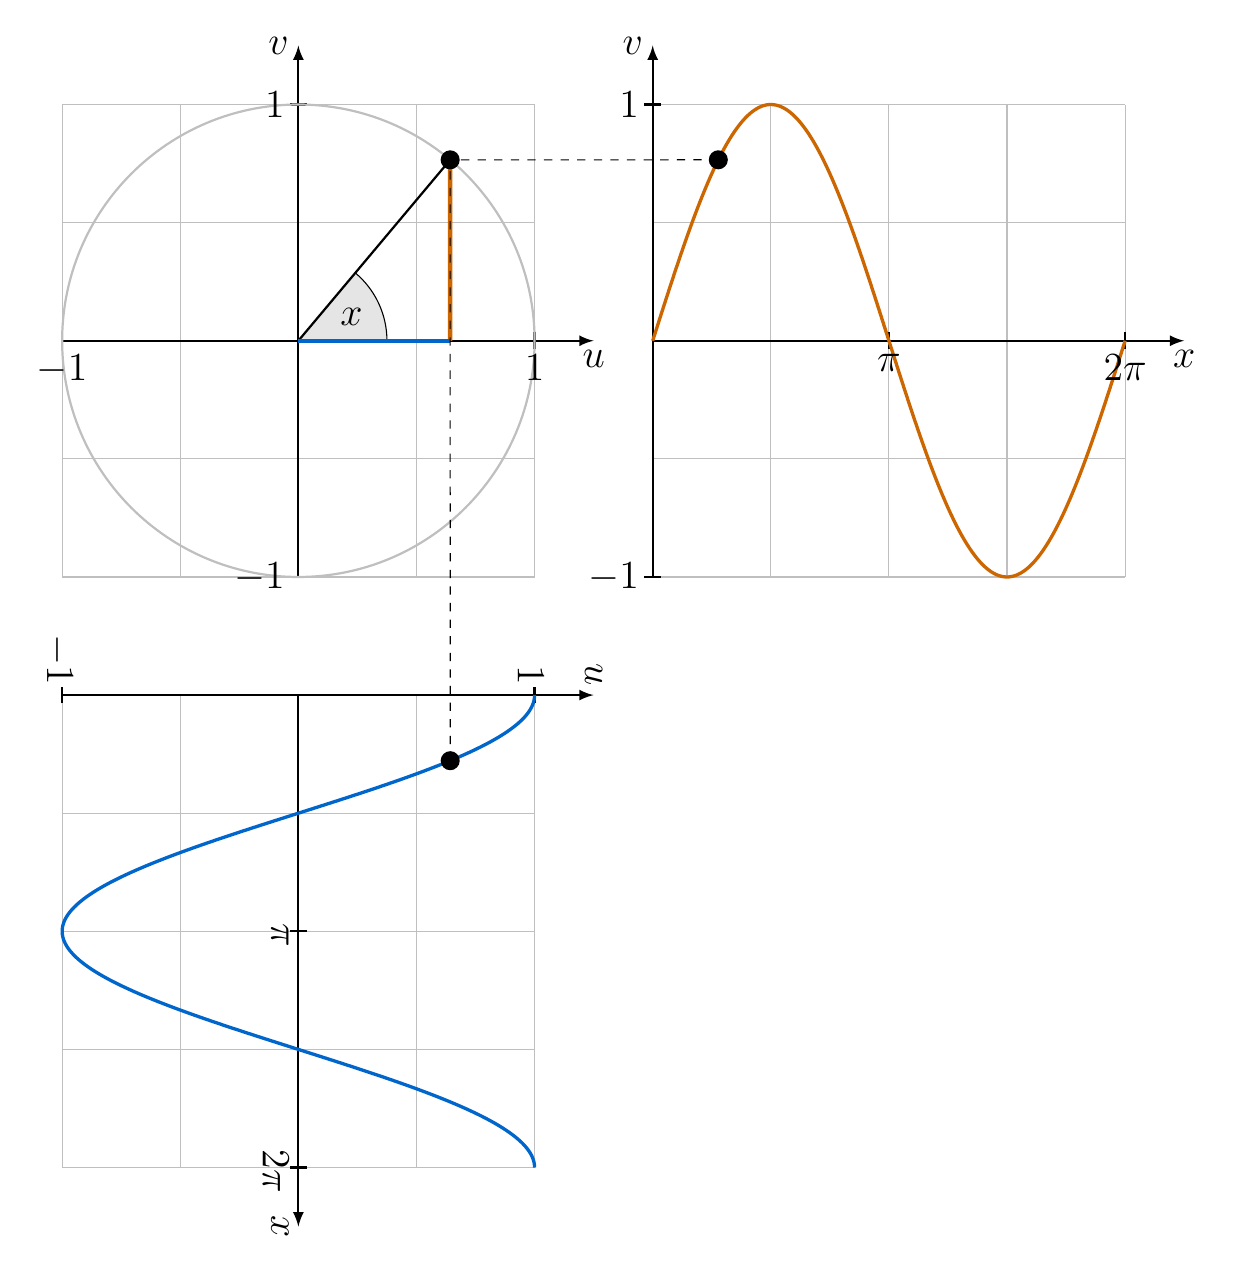
\begin{tikzpicture}[scale=1.5, font=\Large]
			\tkzDefPoint(2*cos(10*pi/36),2*sin(10*pi/36)){A}
			\tkzGrid[color=lightgray] (-2,-2)(2,2)
			\tkzGrid[color=lightgray] (3,-2)(7,2)
			\tkzGrid[color=lightgray] (-2,-7)(2,-3)
			\draw[thick, -latex] (-2,0) -- (2.5,0);
			\draw[thick, -latex] (-2,-3) -- (2.5,-3);
			\draw[thick, -latex] (3,0) -- (7.5,0);
			\draw[thick, -latex] (0,-2) -- (0,2.5);
			\draw[thick, -latex] (3,-2) -- (3,2.5);
			\draw[thick, -latex] (0,-3) -- (0,-7.5);
			\draw[thick] (-2,-0.07) -- (-2,0.07);
			\draw[thick] (2,-0.07) -- (2,0.07);
			\draw[thick] (-2,-3.07) -- (-2,-2.93);
			\draw[thick] (2,-3.07) -- (2,-2.93);
			\draw[thick] (5,-0.07) -- (5,0.07);
			\draw[thick] (7,-0.07) -- (7,0.07);
			\draw[thick] (-0.07,2) -- (0.07,2);
			\draw[thick] (-0.07,-2) -- (0.07,-2);
			\draw[thick] (-0.07,-5) -- (0.07,-5);
			\draw[thick] (-0.07,-7) -- (0.07,-7);
			\draw[thick] (2.93,2) -- (3.07,2);
			\draw[thick] (2.93,-2) -- (3.07,-2);
			\draw[thick, lightgray] (0,0) circle (2 cm);
			\draw[fill,fill opacity=0.1] (0,0) -- (0.75,0) arc (0:50:0.75);
			\draw[very thick,domain=0:360, smooth, samples=300, variable=\x,myorange] plot (3+\x/90, {2*sin(\x)});
			\draw[very thick,domain=0:360, smooth, samples=300, variable=\x,myblue] plot ({2*cos(\x)},-3-\x/90);
			\draw[thick] (0,0) -- (A);
			\draw[ultra thick, myorange] ({2*cos(50)},0) -- (A);
			\draw[ultra thick, myblue] (0,0) -- ({2*cos(50)},0);
			\draw[dashed] ({32/9},{2*sin(50)}) -- (A);
			\draw[dashed] ({2*cos(50)},{-32/9}) -- (A);
			\node[very thick, draw, circle,fill,inner sep=2] at (A) {};	
			\node[very thick, draw, circle,fill,inner sep=2] at ({32/9},{2*sin(50)}) {};	
			\node[very thick, draw, circle,fill,inner sep=2] at ({2*cos(50)},{-32/9}) {};	
			\node[above] at (0.45,0.05){$x$};
			\node[below] at (2.5,0){$u$};
			\node[left] at (0,2.5){$v$};
			\node[left] at (3,2.5){$v$};
			\node[left=0.5mm] at (0,2){$1$};
			\node[left=0.5mm] at (0,-2){$-1$};
			\node[left=0.5mm] at (3,2){$1$};
			\node[left=0.5mm] at (3,-2){$-1$};
			\node[below] at (7.5,0){$x$};
			\node[below=0.5mm] at (7,0){$2\pi$};
			\node[below=0.5mm] at (5,0){$\pi$};
			\node[below=0.5mm] at (2,0){$1$};
			\node[below=0.5mm] at (-2,0){$-1$};
			\node[below, rotate=270] at (0,-7.5){$x$};
			\node[below=0.5mm, rotate=270] at (0,-5){$\pi$};
			\node[below=0.5mm, rotate=270] at (0,-7){$2\pi$};
			\node[left, rotate=270] at (2.5,-3){$u$};
			\node[left=0.5mm, rotate=270] at (2,-3){$1$};
			\node[left=0.5mm, rotate=270] at (-2,-3){$-1$};
	\end{tikzpicture}	
\end{document}
